\documentclass[12pt,a4paper]{article}
\usepackage[utf8]{inputenc}
\usepackage[russian]{babel}
\usepackage[OT1]{fontenc}
\usepackage{mathtools}
\usepackage{amsfonts}
\usepackage{amssymb}
\usepackage{enumitem}
\usepackage{alltt}
\usepackage{graphicx}
\usepackage{indentfirst}
\usepackage{caption}
\usepackage{float}
\usepackage{wrapfig}
\setlength{\parindent}{0.75cm}
\graphicspath{{pictures/}}
\DeclareGraphicsExtensions{.png}
\usepackage[left=15mm,right=15mm,top=2cm,bottom=2cm]{geometry}
\author{Глотов Алексей}
\begin{document}
\newpage
\begin{center}
\footnotesize{{ГОСУДАРСТВЕННОЕ АВТОНОМНОЕ ОБРАЗОВАТЕЛЬНОЕ УЧРЕЖДЕНИЕ}\break
{ВЫСШЕГО ОБРАЗОВАНИЯ}
\break
{\bf {МОСКОВСКИЙ ФИЗИКО-ТЕХНИЧЕСКИЙ ИНСТИТУТ}}
\break
\small{(НАЦИОНАЛЬНЫЙ ИССЛЕДОВАТЕЛЬСКИЙ УНИВЕРСИТЕТ)}}
\break
\hfill \break
\hfill \break
\begin{center}
\normalsize{Кафедра общей физики}
\end{center}
\hfill \break
\hfill \break
\hfill \break
\hfill \break

\begin{center}
\normalsize {Лабораторная работа 2.5.1}
\end{center}
\hfill \break\\
\large{Измерение коэффициента поверхностного натяжения жидкости}
\end{center}
\begin{flushleft}
\hfill \break
\hfill \break
\hfill \break
\hfill \break
\hfill \break
\hfill \break
\hfill \break
\hfill \break
\hfill \break
\hfill \break
\hangindent=9cm
\normalsize{Преподаватель:}\hfill
\normalsize{доцент Игуменов А.Ю.}\\
\hfill \break
\normalsize{Обучающийся:}\hfill
\normalsize{Глотов А.А} \\
\hfill \break
\end{flushleft}
\hfill \break
\hfill \break
\hfill \break
\hfill \break
\hfill \break
\hfill \break
\hfill \break
\hfill \break
\hfill \break
\hfill \break
\hfill \break

\begin{center}
Долгопрудный \break
 2022
\end{center}
\thispagestyle{empty}
\newpage
\section{Введение}

\subsection{Аннотация}

Данная работа посвящена изучению явления поверхностного натяжения жидкостей. В работе используются следующие методы: построение и анализ графика зависимости p(T), пересчитанный из значений показания манометра.


\textbf{Цель работы:}  \begin{enumerate}
	\item измерение температурной зависимости  коэффициента поверхностного натяжения дистиллированной воды с использованием известного коэффициента поверхностного натяжения спирта;
	\item определение полной поверхностной энергии  и теплоты, необходимой для изотермического образования единицы  поверхности жидкости  при различной температуре.
\end{enumerate}

\textbf{В работе используются:} прибор  Ребиндера  с термостатом и микроманометром; исследуемые жидкости; стаканы; микроскоп.
\subsection{Теоретические сведения}

Наличие поверхностного слоя приводит к различию давлений по разные стороны от искривленной границы раздела двух сред.  Для сферического пузырька с воздухом  внутри жидкости избыточное давление даётся формулой Лапласа:

\begin{equation}\label{key}
\Delta P = P_{int} - P_{ext} = \frac{2\sigma}{r},
\end{equation}
где $ \sigma $ -- коэффициент поверхностного натяжения, $ P_{int} $ и $ P_{ext} $ -- давление внутри пузырька и снаружи, $ r $ -- радиус кривизны поверхности раздела двух фаз. Эта формула лежит в основе предлагаемого метода определения коэффициента поверхностного натяжения жидкости. Измеряется давление $ \Delta P $, необходимое для выталкивания в жидкость пузырька воздуха.

\subsection{Схема эксперимента}


Поверхностное натяжение можно определить по величине разряжения $ \Delta P $ \eqref{key}, необходимого для прохождения пузырьков (при известном радиусе иглы).

Разряжение в системе создается с помощью аспиратора $ A $. Кран $ K_2 $ разделяет две полости аспиратора. Верхняя полость при закрытом кране $ K_2 $ заполняется водой. Затем кран $ K_2 $ открывают и заполняют водой  нижнюю полость  аспиратора.  Разряжение воздуха создается в нижней полости  при открывании крана $ K_1 $, когда  вода вытекает из неё по каплям. В колбах $ В $ и $ С $, соединённых трубками с нижней полостью аспиратора, создается такое же пониженное давление. Разность давлений в полостях с разряженным воздухом и атмосферой измеряется спиртовым микроманометром. 

Для стабилизации температуры исследуемой жидкости через рубашку $ D $ колбы $ В $ непрерывно прогоняется вода из термостата.

\subsection{Методика измерений}

Обычно кончик иглы лишь касается поверхности жидкости, чтобы исключить влияние гидростатического давления столба жидкости. Однако при измерении температурной зависимости коэффициента поверхностного натяжения возникает ряд сложностей. Во-первых, большая теплопроводность металлической трубки приводит к тому, что температура на конце трубки заметно ниже, чем в глубине жидкости. Во-вторых, тепловое расширение поднимает уровень жидкости при увеличении температуры.

Обе погрешности можно устранить, погрузив кончик трубки до самого дна. Полное давление, измеренное при этом микроманометром, равно \[ P = \Delta P + \rho g h.\] Заметим, что $ \rho gh $ от температуры практически не зависит, так как подъём уровня жидкости компенсируется уменьшением её плотности (произведение $ \rho g $ определяется массой всей жидкости и поэтому постоянно). Величину  $ \rho g h $ следует измерить двумя способами.

Во-первых, замерить величину $ P_1= \Delta P' $, когда кончик трубки только касается поверхности жидкости. Затем при этой же температуре опустить иглу до дна и замерить $ P_2= \rho gh + \Delta P'' $ ($ \Delta P' $, $ \Delta P'' $ -- давление Лапласа). Из-за  несжимаемости  жидкости можно положить $ \Delta P' = \Delta P'' $ и тогда 

\begin{equation}
 \rho gh= P_2 - P_1. 
\end{equation}
 
Во-вторых, при измерениях $ P_1 $ и $ P_2 $ замерить линейкой  глубину погружения иглы $ h $. Это можно сделать, замеряя расстояние между верхним концом иглы и любой неподвижной частью прибора при положении иглы на поверхности и в глубине колбы.

\subsection{Экспериментальная установка}

\begin{figure}[H]
	\begin{center}
		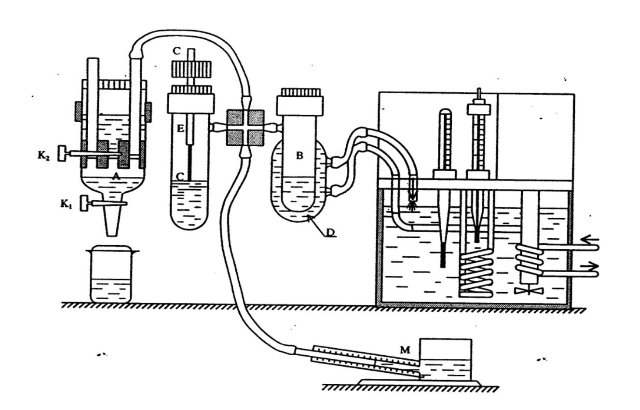
\includegraphics[width=15cm]{2.5.1_1}
		\caption{Рисунок экспериментальной установки}\label{img:ust}
	\end{center}
\end{figure}

Исследуемая жидкость (дистиллированная вода) наливается в сосуд (колбу) $ B $ (рис. \ref{img:ust}). Тестовая жидкость  (этиловый спирт) наливается  в сосуд $ E $.  При измерениях  колбы герметично закрываются  пробками. Через одну из двух пробок  проходит полая металлическая игла $ С $. Этой пробкой закрывается сосуд, в котором  проводятся измерения. Верхний конец иглы открыт в атмосферу, а нижний погружен в жидкость. Другой сосуд герметично закрывается второй пробкой. При создании достаточного  разряжения воздуха в колбе с иглой пузырьки воздуха начинают пробулькивать через жидкость. 

\newpage

\section{Результаты измерений и обработка данных}

\subsection{Измерение диаметра иглы}

Измерим максимальное давление $ \Delta P $  при  пробулькивании пузырьков воздуха через спирт. Результаты измерений занесём в таблицу.

\begin{center}
\begin{tabular}{|c|c|c|c|c|c|}
\hline 
№ эксперимента & 1 & 2 & 3 & 4 & 5 \\ 
\hline 
h, мм & 43 & 43 & 43 & 43 & 43 \\ 
\hline 
p, Па & 67,8 & 67.8 & 67.8 & 67.8 & 67.8 \\
\hline
\end{tabular} 
\end{center}

Учтём, что показания микроманометра связаны с давлением следующим соотношением:  

\begin{equation}
P=h \cdot 0,2 \cdot 9,8 \cdot 805
\end{equation}

 где 0.805 -- плотность спирта, определяемая при данной температуре по паспорту прибора, а константы 0,2 и 9,8 являются константами работы, связывающие наклон манометра с законом гидростатического давления 

Отметим, что расхождения в результатах измерения не наблюдается, что говорит о малости случайной погрешности по сравнению с приборной, а полная погрешность будет определяться только погрешностью прибора

Систематическую погрешность определим из расчёта, что погрешность измерения составила $ 1 $ деление прибора, или же {$ \sigma_{P}^\text{сист} \approx 1,6 $ Па}.

Полная погрешность измерений определяется по формуле:

\begin{equation}\label{full_pogr}
\sigma_{P}=\sqrt{(\sigma_{P}^\text{сист})^2 + (\sigma_{P}^\text{случ})^2} \approx \sigma_{P}^\text{сист} = 1.6 \text{ Па}.
\end{equation}

Итого получаем { $ \Delta P = (63.5 \pm 1.6) \text{ Па},$} \quad $(\varepsilon = 2,5 \%) $.


Согласно табличным данным, коэффициент поверхностного натяжения этилового спирта при комнатной температуре равен $ \sigma_{alc} = 22,4 $ мН/м. По полученным результатам измерения и при помощи \eqref{key} вычисляем диаметр иглы по формуле:

\label{diametr}

\begin{equation}\label{igla}
d=\frac{4\sigma}{\Delta P} \approx 1,41 \text{ мм}.
\end{equation}

Также вычисляем погрешность полученного результата:

\begin{equation}\label{igla_pogr}
\sigma_d=d\cdot\varepsilon_{\Delta P_{alc}} \approx 0,04 \text{ мм}.
\end{equation}

Таким образом, получаем окончательный результат измерения диаметра иглы косвенным способом:
\begin{itemize}
	\item ${ d = (1,41 \pm 0,04) \text{ мм},} \: (\varepsilon = 2,5\%). $
\end{itemize}

Проведём измерение диаметра иглы при помощи оптического микроскопа.

По результатам прямого измерения получаем $ {d = (1,10 \pm 0,05) \text{ мм}}, \: (\varepsilon = 4,5\%) $.



\subsection{Определения поправки при измерении давления для погруженной в воду иглы}

Перенесём предварительно промытую и просушенную от спирта иглу в колбу с дистиллированной водой. Измерим максимальное давление $ P_1 $ при пробулькивании пузырьков, когда игла лишь касается поверхности воды. Измерите расстояние между верхним концом иглы и любой неподвижной часть прибора $ h_1 $.

Утопим иглу в воду. Измерим $ h_2 $. Также измерим максимальное давление в пузырьках $ P_2 $. Полученные результаты запишем.

\begin{center}
\begin{tabular}{|c|c|c|}
\hline 
H, мм & 25.0 & 7.0 \\ 
\hline 
h, мм & 106 & 215 \\
\hline
p, Па & 166.6 & 339.5 \\ 
\hline 
\end{tabular} 
\end{center}

Отметим, что все данные снимались по 5 измерений, но в связи с малостью случайной погрешностью по сравнению с приборной (значения всех измерений одинаковы), в таблицу заносилось только среднее значение

Исходя из экспериментальных данных, определяем среднее значение давления $ \langle P \rangle $ и погрешность измерения $ \sigma_{P} $ по формулам (1), (2) и (3).

По полученным данным определяем \[ P_2-P_1 = 172.9 \text{ Па}. \]

Также вычисляем погрешность:  \begin{equation}\label{pogr_sum}
\sigma_{\Delta P} = \sqrt{\sigma^2_{P_1}+\sigma^2_{P_2}} \approx 2,3 \text{ Па}.
\end{equation}

Таким образом, получаем $ {\Delta P = (172,9 \pm 2,3) \text{ Па},} \: (\varepsilon = 1,3\%).$

По полученному значению $ \Delta P $ можем рассчитать $ \Delta h $ по следующей формуле: \[ \Delta h = \frac{\Delta P}{\rho g} \approx 17,6 \text{ мм}, \] где $ \rho = 1000 $ кг/$ \text{м}^3 $ -- плотность воды и $ g = 9,8 $ м/$ \text{с}^2 $ -- ускорение свободного падения.

\medskip

При этом погрешность нашего измерения равна \[ \sigma_{\Delta h} = \Delta h \cdot \varepsilon_{\Delta P} \approx 0,2 \text{ мм}. \]

Таким образом, получаем $ {\Delta h = (17,6 \pm 0,2) \text{ мм}}, \: (\varepsilon = 1,1\%). $

По результатам измерений, необходимая поправка будет $\Delta{P} = (172.5 \pm 1.9)$ Па

\subsection{Измерение температурной зависимости коэффициента поверхностного натяжения}

Снимем температурную зависимость $ \sigma(T) $ дистиллированной воды. 

Исходя из экспериментальных данных, определяем среднее значение давления $ \langle P' \rangle $ и погрешность измерения $ \sigma_{P'} $ 

Учтём поправку к измеренному давлению, которая была вычислена в \ref{popravka}. Полученные результаты также заносим в таблицу.


\begin{center}
\begin{tabular}{|c|c|c|c|c|c|}
\hline 
T, K & h, мм & $P^{'}$, Па & P, Па & $\sigma, \frac{\text{мН}}{\text{м}}$ & $\sigma_{\sigma},\frac{\text{мН}}{\text{м}} $ \\ 
\hline 
298 & 217 & 342,4 & 169.5 & 46.6 & 2.1 \\ 
\hline 
303 & 216 & 340,8 & 167.9 & 46.2 & 2.1 \\ 
\hline 
308 & 215 & 339,2 & 166.3 & 45.7 & 2.1 \\ 
\hline 
313 & 214 & 337,6 & 164.7 & 45.3 & 2.0 \\ 
\hline 
318 & 213 & 336,1 & 163.2 & 44.9 & 2.0 \\ 
\hline 
323 & 212 & 334,5 & 161.6 & 44.4 & 2.0 \\ 
\hline 
328 & 211 & 332,9 & 160.0 & 44.0 & 2.0 \\ 
\hline 
333 & 210 & 331,3 & 158.4 & 43.6 & 2.0 \\ 
\hline 
\end{tabular} 
\end{center}

Отметим, что все данные снимались по 5 измерений, но в связи с малостью случайной погрешностью по сравнению с приборной (значения всех измерений одинаковы), в таблицу заносилось только среднее значение

По полученным данным вычислим коэффициент поверхностного натяжения для каждой из температур по формуле

\begin{equation}\label{sigma}
\sigma = \frac{Pd}{4},
\end{equation}
где $ d $ -- диаметр иглы, вычисленный в \ref{diametr}. Погрешность такого результата вычисляется по следующей формуле:

\begin{equation}\label{otn_pogr}
\sigma_\sigma = \sigma\sqrt{\varepsilon^2_P + \varepsilon^2_d}.
\end{equation}

Полученные результаты заносим в таблицу.


\begin{figure}[H]
	\begin{center}
		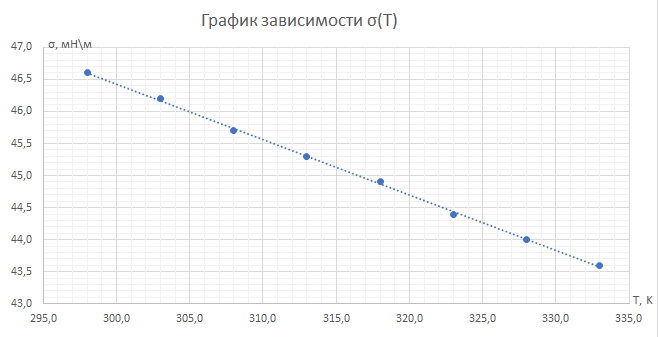
\includegraphics[width=14cm]{2.5.1_gr_1}
	\end{center}
\end{figure}


Полученную зависимость наносим на график. Вычислим коэффициенты аппроксимирующей прямой $ \sigma = kT + b $, где $ \displaystyle k = \frac{d\sigma}{dT} $, используя метод наименьших квадратов:

\[ k = \frac{\langle T\sigma \rangle - \langle T \rangle \langle \sigma \rangle}{\langle T^2 \rangle - \langle T \rangle ^2} \approx -0,086\text{ } \frac{\text{мН}}{\text{м}\cdot\text{К}},\]

\[ b = \langle \sigma \rangle - k\langle T \rangle \approx 72,4\text{ } \frac{\text{мН}}{\text{м}}. \]

Случайные погрешности определения этих коэффициентов вычислим по следующим формулам:

\[ \sigma^\text{случ}_k = \sqrt{\frac{1}{N-2} \left(\frac{\left\langle\left(\sigma - \langle \sigma\right\rangle\right)^2 \rangle}{\left\langle\left(T - \langle T\right\rangle\right)^2 \rangle}\right)-k^2} \approx 0,003 \text{ } \frac{\text{мН}}{\text{м}\cdot\text{К}},\]

\[ \sigma^\text{случ}_b=\sigma^\text{случ}_k\sqrt{\left\langle x^2 \right\rangle} \approx 1,2\text{ } \frac{\text{мН}}{\text{м}}. \]

Систематические погрешности оценим по следующим формулам:

\[ \sigma^\text{сист}_k = |k|\sqrt{\varepsilon^2_T+\varepsilon^2_\sigma} \approx |k|\varepsilon_{\sigma} = 0,004 \text{ } \frac{\text{мН}}{\text{м}\cdot\text{К}}, \]
\[ \sigma^\text{сист}_b = b\sqrt{\varepsilon^2_T+\varepsilon^2_\sigma} \approx b\varepsilon_{\sigma} = 2,8 \text{ } \frac{\text{мН}}{\text{м}}. \]

Таким образом, полные погрешности измерений определяются следующими соотношениями:
\[ \sigma_k = \sqrt{(\sigma_k^\text{сист})^2 + (\sigma_k^\text{случ})^2} \approx 0,006 \text{ } \frac{\text{мН}}{\text{м}\cdot\text{К}},\]
\[ \sigma_b = \sqrt{(\sigma_b^\text{сист})^2 + (\sigma_b^\text{случ})^2} \approx 3,3 \text{ } \frac{\text{мН}}{\text{м}}. \]

Таким образом, окончательно получаем:
\begin{itemize}
	\item $ \displaystyle {k = \frac{d\sigma}{dT} = (-0,086 \pm 0,005) \text{ } \frac{\text{мН}}{\text{м}\cdot\text{К}}, \: (\varepsilon = 5.8\%);} $
	\item $ \displaystyle {b = (72,4 \pm 3,0) \text{ } \frac{\text{мН}}{\text{м}}, \: (\varepsilon = 4,2\%).}$
\end{itemize}

По полученным данным получим зависимости от температуры коэффициента поверхностного натяжения,  теплоты образования единицы поверхности жидкости $ \displaystyle {q = -T\frac{d\sigma}{dT}} $ и поверхностной энергии $ U $ единицы площади $ F $: $ \displaystyle {\frac{U}{F} = \left(\sigma - T \frac{d\sigma}{dT}\right).} $


\begin{figure}[H]
	\begin{center}
		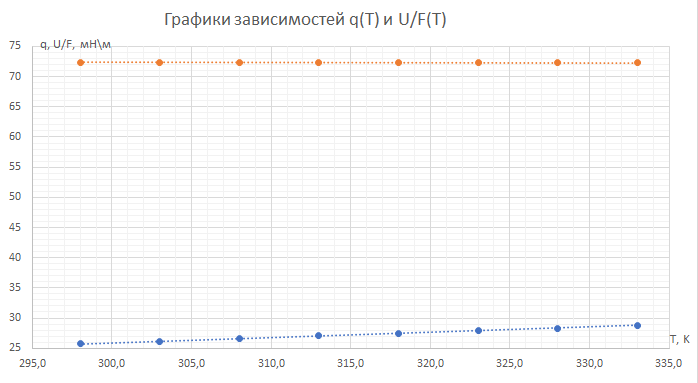
\includegraphics[width=14cm]{2.5.1_gr_2}
	\end{center}
\end{figure}

\newpage

\section{Обсуждение результатов и выводы}

В ходе работы были достигнуты следующие цели:
\begin{itemize}
\item Различными способами измерен диаметр иглы, используемой в работе
\item Экспериментально подтверждено существование явления поверхностного натяжения жидкостей
\item Экспериментально получены и обработаны зависимости коэффициента поверхностного натяжения, теплоты образования единицы поверхности жидкости и поверхностной энергии на единицу площади от температуры.
\end{itemize}

В ходе работы с неплохой точностью (4,5\% и 1,1 \%) были получены значения внутреннего диаметра иглы, используемой в работе. Следует отметить, что несмотря на близость результатов, они не лежат в пределах погрешности друг друга.($(1,41 \pm 0.04)$ и $(1.10 \pm 0.05)$ мм), что говорит о том, что в первом методе не были учтены какие-то величины и явления, и метод требует дополнительного внимания

Также в ходе работы были определено значение коэффициента поверхностного натяжения анилина. Табличное значения при комнатной температуре равно $42.9 \frac{\text{мН}}{м}$. Полученное нами значение равно $(46.6 \pm 2.1 \frac{\text{мН}}{м})$. Видно, что значения достаточно близки друг к другу, а расхождения можно списать, например, на наличие примесей воды в анилине.

Нами была установлены зависимости 3 величин от температуры (см. достигнутые цели). Для каждой из них была подтверждена линейная зависимость с сохранением предсказанного теоретически характера монотонности (убывание, возрастание и постоянная величина; перечисление в порядке, указанном в достигнутых целях)

\end{document}